\PassOptionsToPackage{pdfpagelabels=false}{hyperref}
\documentclass[fleqn,usenatbib,usedcolumn]{mnras}
%==============================================================================%
\usepackage[british]{babel}             % British English hyphenation
\usepackage{txfonts}                  % Good fonts
% Use vector fonts, so it zooms properly in on-screen viewing software
% Don't change these lines unless you know what you are doing
%\usepackage[T1]{fontenc}
%\usepackage{ae,aecompl}
%%%%% AUTHORS - PLACE YOUR OWN PACKAGES HERE %%%%%
\usepackage{graphicx}	% Including figure files
\usepackage{hyperref} % hyperlinks
\usepackage{natbib}
\usepackage{aastexmacros}
\usepackage{tikz}
\usepackage[caption=false]{subfig}
%%%%%%%%%%%%%%%%%%%%%%%%%%%%%%%%%%%%%%%%%%%%%%%%%%

%%%%% AUTHORS - PLACE YOUR OWN COMMANDS HERE %%%%%
\usetikzlibrary{shapes,arrows,calc,positioning}

\newcommand{\text}{\mathrm}
\newcommand{\cheng}[1]{ {\color{teal}[{\bf Cheng:~{#1}}]} }

%%%%%%%%%%%%%%%%%%%%%%%%%%%%%%%%%%%%%%%%%%%%%%%%%%

%%%%%%%%%%%%%%%%%%% TITLE PAGE %%%%%%%%%%%%%%%%%%%

\title[ML CDFS]{Radio Galaxy Zoo: Machine learning methods for radio host cross-identification}

\author[RGZ ML Team]{M. J. Alger$^{1}$, J. K. Banfield$^{1, 2}$, C. S. Ong$^{3}$, O. I. Wong$^{2, 4}$, others
\\
% List of institutions
$^{1}$Research School of Astronomy and Astrophysics, The Australian National University, Canberra ACT 2611, Australia\\
$^{2}$ARC Centre of Excellence for All-Sky Astrophysics (CAASTRO)\\
$^{3}$Data61, CSIRO, 7 London Circuit, Canberra ACT 2601, Australia\\
$^{4}$International Centre for Radio Astronomy Research-M468, The University of Western Australia, 35 Stirling Hwy, Crawley, WA 6009, Australia
}

% These dates will be filled out by the publisher
\date{Accepted XXX. Received XXX}

% Enter the current year, for the copyright statements etc.
\pubyear{2017}

% Don't change these lines
\begin{document}
\label{firstpage}
\pagerange{\pageref{firstpage}--\pageref{lastpage}}
\maketitle

% Abstract of the paper
\begin{abstract}
  We present a machine learning approach for radio host cross-identification,
  the task of determining the host galaxies of radio emissions detected in
  wide-area radio surveys. Training a machine learning algorithm requires a
  large amount of labelled training data, which can be difficult or expensive
  to acquire. Radio Galaxy Zoo, a citizen science project on the Zooniverse
  platform, provides a large number of radio host cross-identifications which
  may be used as labels for training. However, these cross-identifications are
  assigned by non-experts, and may be incorrect. We find that while machine
  learning algorithms trained on expert labels outperform those trained on the
  crowdsourced Radio Galaxy Zoo labels, the accuracies are comparable and the
  crowdsourced labels are still useful for training. [TODO: add balanced
  accuracies]
\end{abstract}

% Select between one and six entries from the list of approved keywords.
% Don't make up new ones.
\begin{keywords}
galaxies: active -- galaxies: clusters -- radio continuum: galaxies
\end{keywords}

%%%%%%%%%%%%%%%%%%%%%%%%%%%%%%%%%%%%%%%%%%%%%%%%%%
%%%%%%%%%%%%%%%%% BODY OF PAPER %%%%%%%%%%%%%%%%%%

\section{Introduction}\label{introduction}

  \cheng{Avoid using words like simple, easy, obvious, etc.}

  Next generation radio telescopes such as the Australian SKA Pathfinder
  \citep[ASKAP;][]{johnston07} and Apertif \citep{verheijen08} will
  conduct increasingly wide, deep, and high-resolution surveys. These
  surveys will produce very large amounts of data. The Evolutionary Map of
  the Universe survey \citep[EMU;][]{norris11} using ASKAP and the WODAN
  survey \citep{rottgering11} using Apertif are expected to detect
  over 100 million radio sources between them, compared to the 2.5 million
  radio sources already known \citep{banfield15}.

  An important part of processing this data is cross-identifying observed
  radio emission regions with observations of their host galaxy in surveys at
  other wavelengths. Radio host cross-identification is a difficult task.
  While pointlike sources of radio emission are easy to cross-identify as they
  directly overlap the host galaxy, a large proportion of radio sources are
  considerably more complex. Radio emissions from radio-loud active galactic
  nuclei (AGN) may be complicated structures not clearly related to the host
  galaxy, and are often composed of multiple, separate components. These AGN
  are expected to dominate approximately 30\% of sources detected by EMU
  \citep{norris11}. Small surveys of a few thousand sources such as the
  Australia Telescope Large Area Survey
  \citep[ATLAS;][]{norris06,middelberg08} can be cross-identified manually,
  but this is impractical for larger surveys.

  One approach to cross-identification is crowdsourcing, where members of the
  public volunteer to cross-identify radio emissions with their host galaxies.
  This is the premise of Radio Galaxy Zoo \citep[RGZ;][]{banfield15}, a
  citizen science project hosted on the highly successful Zooniverse platform
  \citep{lintott08}. Volunteers are shown images of the radio sky, and are
  asked to identify the morphology of radio sources in each image. They are
  then asked to cross-identify each radio source with its host galaxy in a
  corresponding infrared image. Radio Galaxy Zoo provides a large dataset of
  100~267 radio host cross-identifications and radio source morphologies (Wong
  et al., 2017). While this is a much larger number of cross-identifications
  than have been made by experts, it is still far short of the millions of
  radio sources expected to be detected in upcoming surveys.

  Automated algorithms have been developed for this cross-identification
  problem. \citet{fan15} developed a method of cross-identification using
  Bayesian hypothesis testing, fitting a three-component model to extended
  radio sources under the assumption that radio sources are composed of a core
  radio component and two lobe components. The core radio component is
  coincident with the host galaxy, so cross-identification amounts to finding
  the galaxy coincident with the core in the most likely model fit. This
  method is easily extended to use other, more complex models, but it is
  purely geometric and does not incorporate other information such as the
  colours of the potential host galaxy. Additionally, there may be new classes
  of radio source detected in future surveys like EMU which do not fit the
  model, and it is these radio sources that are of most interest.
  \citet{weston17} developed a modification of the likelihood ratio method of
  cross-identification \citep{richter75} for application to EMU. However, this
  method is only intended to cross-identify ``simple'' sources consisting of a
  single, isolated radio component \citep{norris17unexpected}. [TODO(Julie):
  Can you elaborate on this?]

  ASKAP is expected to generate approximately 70 PB yearly
  \citep{norris17unexpected}. Automated methods will be needed to choose what
  data to keep and what to discard. While data can be selected for
  preservation by model-based methods, it is clear that these methods would
  miss the unexpected objects we expect to find in EMU [TODO: Discuss with
  Julie inclusion of a WAT example here.]. EMU will therefore need to employ
  an algorithm for looking for these unexpected objects
  \citep{norris17unexpected}, which may be of the form of an outlier detector.
  Outliers can be detected in a variety of ways, including imposing a
  similarity metric on radio components and looking for objects very distant
  from other objects \citep{polsterer15pink}, looking for objects that do not
  reliably fit existing models \citep[potentially an extension of][]{fan15},
  or generating a model of radio galaxies from existing data and looking for
  objects that do not fit this model. These methods all require a way of
  encoding objects, a process called \emph{feature selection}. Given that EMU
  is expected to find unusual objects, robust feature selection is important.
  Model-based approaches \citep[e.g.][]{proctor06} will likely fail. [TODO: Discuss with Julie whether we even need this paragraph.]

  {[}TODO: literature review: paper Ivy sent, PINK, WTF, Fan (done),
  Proctor, Park et al. 2017{]}

  {[}TODO: Note that outlier detection can be done in lots of different
  ways including with this work and there are benefits in both. Also an
  example of where model-based approaches fall down. Elaborate on this?{]}

  In order to investigate methods for efficiently and effectively classifying
  radio galaxy hosts for upcoming large radio surveys, we have developed a
  machine learning approach for radio host cross-identification using standard
  machine learning techniques.

  \begin{figure}
    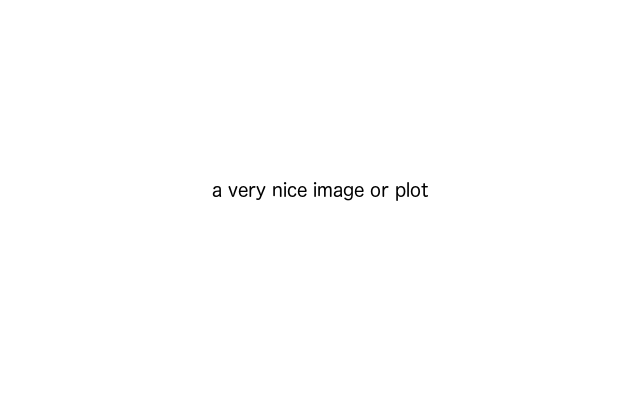
\includegraphics[width=\linewidth]{images/placeholder.png}
    \caption{[TODO: Define component, source, primary component, host, in a figure.]}
  \end{figure}

\section{Data}\label{data}

  \subsection{Radio Galaxy Zoo}\label{sec:rgz}

    Radio Galaxy Zoo asks volunteers to cross-identify radio components with
    their infrared host galaxies. A total of 177~461 radio components are
    sourced from ATLAS \citep{franzen15} and Faint Images of the Radio
    Sky at Twenty-Centimeters \citep[FIRST;][]{white97first}. These components
    are cross-identified to host galaxies detected in the \emph{Spitzer} Wide-
    Area Infrared Extragalactic survey \citep[SWIRE;][]{lonsdale03swire} and
    by the \emph{Wide-Field Infrared Survey Explorer}
    \citep[WISE;][]{wright10wise}, respectively.

    Volunteers are presented with a random radio image centred on a radio
    component, and a corresponding infrared image centred on the same
    location. The radio image may contain multiple radio components.
    Classification of these images is a two-step process. First, volunteers
    select which radio components are part of the same radio source. Second,
    volunteers associate each radio source with a host galaxy visible in the
    infrared image. A more detailed description can be found in
    \citet{banfield15}.

    To reduce noise, each radio component is shown to multiple volunteers.
    Compact radio components are shown to 5 volunteers, while extended radio
    components are shown to 20 volunteers. Once a radio object has been
    classified by the required number of volunteers, it is considered
    ``complete''. Complete classifications are combined to produce the final
    catalogue of Radio Galaxy Zoo morphologies and cross-identifications. The
    most commonly chosen associations of radio components to radio sources are
    chosen as the radio morphology classification for the image. The host
    galaxy locations selected by volunteers who agreed with the most common
    radio morphology classification are combined by maximising over a kernel
    density estimate of the locations. These locations are then matched to the
    nearest SWIRE object within $3"$. A full description of the catalogue
    generation can be found in \citet{wong17}. As of 30 March 2016, there are
    97~807 complete classifications of FIRST components, and 2460 complete
    classifications of ATLAS components (the latter comprising the entire
    \emph{Chandra} Deep Field - South).

    In this paper we focus on the Radio Galaxy Zoo cross-identifications of
    the ATLAS and SWIRE surveys. There are two main reasons for this. The
    first is that ATLAS is the pilot study for EMU where automated methods
    like ours will be used. The second is that ATLAS is composed of two
    fields, so we can train methods on one field and test these methods on
    the other field to ensure that our methods apply in different areas of
    the sky observed by the same telescope.

    Each primary component found in the ATLAS DR3 component catalogue
    appears in Radio Galaxy Zoo. Non-primary components may appear within
    the image of a primary component, but do not have their own entry in
    Radio Galaxy Zoo. We will henceforth only discuss the primary
    components. For ATLAS components, the radio and infrared images shown to
    volunteers are \(2' \times 2'\).

  \subsection{ATLAS}\label{sec:atlas}

    ATLAS \citep{franzen15} is a wide-area radio survey of the \emph{Chandra}
    Deep Field - South (CDFS) and the ESO Large Area ISO Survey - South 1
    (ELAIS-S1) fields at 1.4 GHz. It is a pilot survey for the EMU
    \citep{norris11} survey that will be conducted with ASKAP. EMU will cover
    the entire southern sky and is expected to detect approximately 70 million
    new radio sources. EMU will be conducted at the same depth and resolution
    as ATLAS, so methods developed for processing ATLAS data are expected to
    work for EMU. [TODO: How large are CDFS and ELAIS-S1? How many radio
    objects do they contain?] ATLAS has a sensitivity of 14 $\mu$Jy on CDFS and
    17 $\mu$Jy on ELAIS-S1. CDFS contains 3034 radio components and ELAIS-S1 contains 2084 radio components above 5$\sigma$ \citep{franzen15}.

    \begin{table}
      \center
      \begin{tabular}{cc|cc}
        Catalogue & Method & \#CDFS & \#ELAIS-S1\\\hline
        \citet{norris06} & Manual & 784 & 0\\
        \citet{middelberg08} & Manual & 0 & 1366\\
        \citet{fan15} & Bayesian models & 784 & 0\\
        \citet{wong17} & Crowdsourcing & 2460 & 1 \\
        \citet{weston17} & Likelihood ratio & 3078 & 2113
      \end{tabular}
      \caption{Catalogues of ATLAS/SWIRE cross-identifications for the CDFS
        and ELAIS-S1 fields. The method used to generate each catalogue is
        shown, along with the number of radio components cross-identified in each
        field.}
      \label{tab:atlas-cids}
    \end{table}

    A number of catalogues have been produced cross-identifying radio components
    in ATLAS and host galaxies in SWIRE. These catalogues are summarised in
    Table \ref{tab:atlas-cids}.

    % \citet{norris06} produced a catalogue of cross-identifications of 784
    % radio sources with their infrared counterparts in SWIRE.
    % \citet{middelberg08} produced a catalogue of cross-identifications of
    % {[}NNNN{]} radio sources with their infrared counterparts in SWIRE.
    % {[}TODO: Make this less clunky and talk about Fan et al.{]}

    % Radio Galaxy Zoo (Section \ref{sec:rgz}) produced a catalogue of
    % crowdsourced cross-identifications of 2460 ATLAS radio objects in CDFS
    % \citep{wong17}.
    % % As these cross-identifications have been based on
    % % volunteer classifications, this catalogue is expected to be less accurate
    % % than an expert catalogue like that produced by \citet{norris06}.

  \subsection{SWIRE}\label{sec:swire}

    The Spitzer Wide-area Infrared Extragalactic survey
    \citep[SWIRE;][]{lonsdale03swire,surace05swire} is a wide-area infrared
    survey at the four IRAC wavelengths 3.6 $\mu$m, 4.5 $\mu$m, 5.8 $\mu$m,
    and 8.0 $\mu$m. It covers eight fields, including CDFS and ELAIS-S1 which
    were also covered by ATLAS. SWIRE is thus the source of infrared
    observations for cross-identification with ATLAS. [TODO: Sensitivity?
    Count?]

  \section{Method}\label{method}

  \subsection{Cross-identification as binary
  classification}\label{cross-identification-as-binary-classification}

    We focus on the problem of cross-identification without reference to radio
    morphology. Given a radio component, we want to find its host galaxy as a
    citizen scientist would using Radio Galaxy Zoo. The input is thus a radio
    image and an infrared image with a given radius. We choose a radius of
    $1'$ to match Radio Galaxy Zoo. We make the assumption that each radio
    image represents a single, complex extended source. This is not the case
    in general and a radio image may contain many different sources. If we had
    access to radio morphology information, we could use this to isolate
    relevant components and hence more accurately cross-identify sources, but
    this is outside the scope of this paper. We also note that this assumption
    will bias our results against radio emission that extends beyond the $1'$
    cutout size. The radio cross-identification task then amounts to locating
    the host galaxy within the associated radio and infrared images. This is
    formalised as an object localisation problem: Given a radio image and an
    infrared image centred on a radio source, locate the host galaxy of the
    radio source.

    \begin{figure}
      \centering
      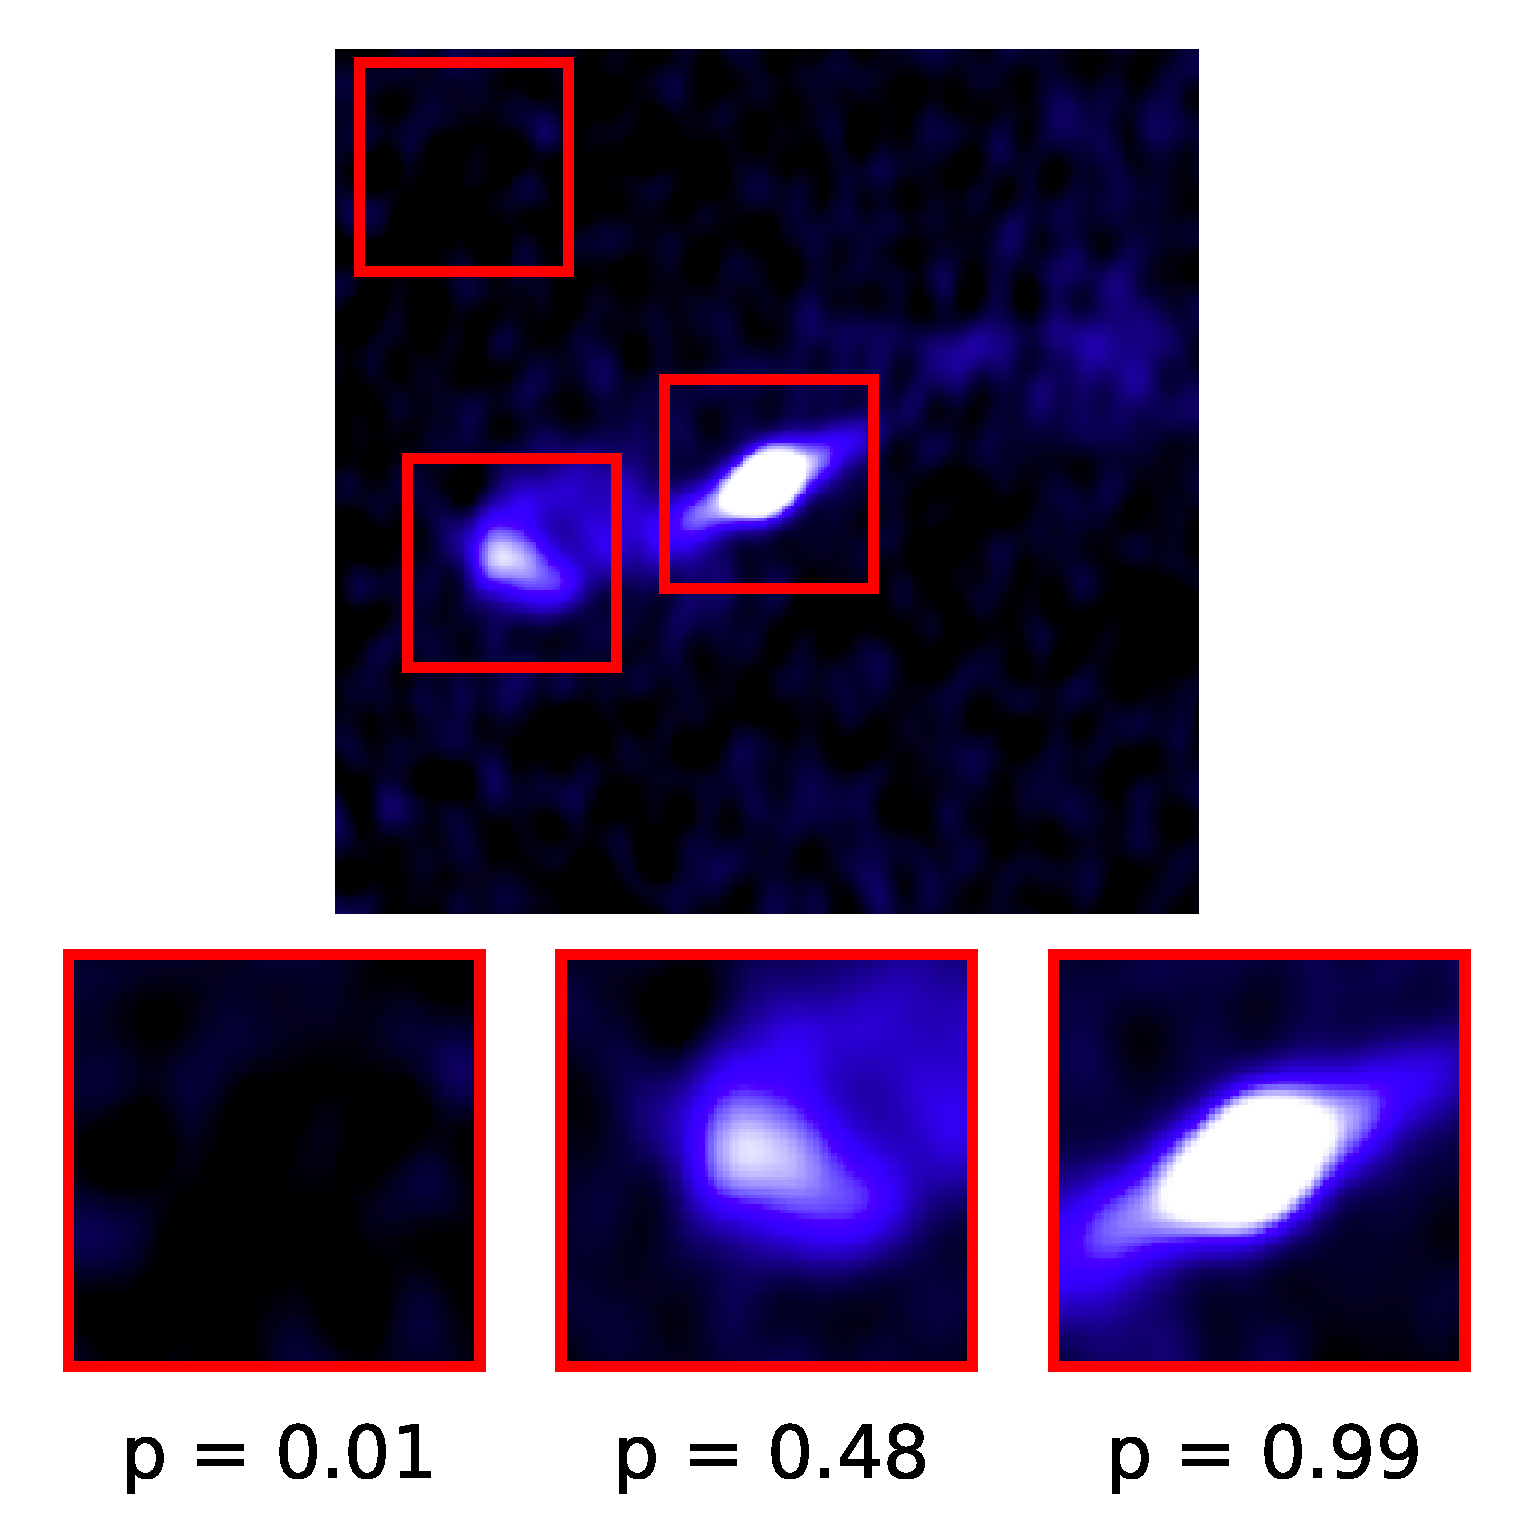
\includegraphics[width=0.8\columnwidth]{images/windows.eps}
      \caption{Localising the host galaxy in a radio image. Red boxes
        represent windows centred on various locations in the image. The image
        patches from each window are shown beneath. The image patch of each
        window represents the location the window is centred on. The
        probabilities of each patch coinciding with the host galaxy would then
        be estimated. The probabilities shown are for illustration only. In
        this example, the centre window of the image would be chosen as the
        location of the host galaxy, as the window centred on it has the
        highest probability. [TODO: Use FITS images]}
      \label{fig:windows}
    \end{figure}

    A common approach to object localisation is to estimate the probability
    that each location in the image is coincident with the desired object. In
    practice this amounts to taking fixed-size windows of the image centred on
    each pixel and estimating the probability that each window is centred on
    the object. The location associated with the highest probability window is
    then assumed to be the location of the object. Applying this to radio host
    cross-identification, we consider windows of a radio/infrared image and
    estimate the probability that each window is centred on the host galaxy.
    This approach is illustrated in Figure \ref{fig:windows}.
    In computer vision a sliding window is commonly used: every possible patch
    in the image is considered.

    \cheng{Make a list of assumptions, then justify them in paragraphs afterwards.
      I suggest a separate subsection ``Limitations of our approach''}

    This task can be made greatly more efficient if we have a prior on the
    location of the object we are localising. For our prior, we assume that
    the host galaxy is always visible in the infrared and thus we only need
    consider windows centred on infrared sources. This assumption usually
    holds, except for a rare class of infrared-faint radio sources. Norris et
    al. (2006) found 22 such radio sources in their sample of 784 bright ATLAS
    components in CDFS. This leads us to a binary classification task: Given
    an infrared source, compute the probability that it is a host galaxy. To
    find the host galaxy given a radio source, classify each galaxy within
    \(R\) of the source and select the galaxy with the highest probability of
    being a host galaxy. This is a good formulation as binary classification
    is a very common problem in machine learning and there are many different
    methods readily available to solve it.

    \cheng{Be careful about the difference between a binary classifier and
      a class probability estimator. $\mathcal{Y}$ can be binary or in the unit interval.}
    Solving the radio cross-identification task amounts to modelling a
    function \(f\) from infrared sources \(\mathcal{X}\) to binary
    \(\mathcal{Y} = \{0, 1\}\): \[
        f : \mathcal{X} \to \mathcal{Y}
    \] There are many options for modelling \(f\). In this paper we apply
    three different models: logistic regression, random forests, and
    convolutional neural networks.
    % As a linear method, logistic regression is
    % the simplest classification approach we can take. Convolutional neural
    % networks have recently shown strong results on image-based classification
    % tasks [TODO: citation needed].

    The space of infrared sources \(\mathcal{X}\) needs to be encoded as a
    vector for the models we will use. We describe this in Section
    \ref{vector-representation-of-infrared-sources}.

    \begin{figure}
      \centering
      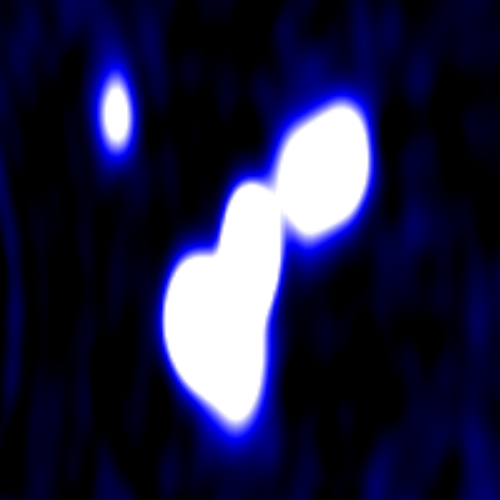
\includegraphics[width=0.5\linewidth]{images/ARG0003r2v_radio.png}
      \caption{$2'$-wide radio image centred on ATLAS3\textunderscore{}J033402.87-282405.8C.
        %(ARG0003r2v)
        This radio source breaks our assumption that there are
        no other sources within $1'$ of the source. Another source is
        visible to the upper-left. [TODO: Use FITS image, describe the colour scaling, include RA and Dec]}
      \label{fig:broken-isolation}
    \end{figure}

    The key problem with this approach is our assumption that the radio sky
    within radius $R$ contains only one, complete radio source. The problem is
    two-fold: This radius may contain multiple sources, or it may not contain
    the entirety of the source. If the radius contains multiple sources then
    there will also be multiple hosts in our input images (which breaks our
    assumption that there is only one); even a perfect classifier can only
    accurately cross-identify \emph{one} host in an image with multiple. An
    example of a radio source that breaks the assumption in this way is shown
    in Figure \ref{fig:broken-isolation}.

    \begin{figure}
      \centering
      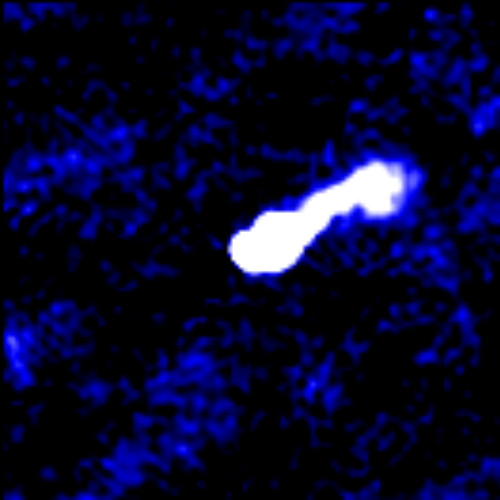
\includegraphics[width=0.45\linewidth]{images/ARG0000u0h_radio.jpg}
      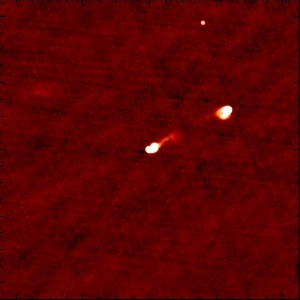
\includegraphics[width=0.45\linewidth]{images/ARG0000u0h_first.jpg}
      \caption{The left image [TODO: a)] is a $3'$-wide radio image from Radio Galaxy
        Zoo, centred on FIRSTJ151227.2+454026. This radio source
        % ARG0000u0h
        breaks our assumption that the whole source is visible in the chosen
        radius. The right image is an $8'$-wide radio image from FIRST centred
        on the same location. In this image, it is clear that the source is a
        radio double. [TODO: Use FITS image (fetch the left image from FIRST
        cutout server), describe the colour scaling, include RA and Dec, use
        subfigures] [TODO: Put a box around the left image in the right image]}
      \label{fig:broken-contains}
    \end{figure}

    If the radius does not contain the whole source, then we are missing radio
    information useful for finding the host galaxy. This is a difficult
    problem even for non-automated methods as radio sources can be extremely
    wide --- for example, Radio Galaxy Zoo found a radio giant that spanned
    over three different images presented to volunteers and the full source
    was only cross-identified by the efforts of citizen scientists
    \citep{banfield15}. An example of a radio image where part of the radio
    source is outside the search radius is shown in Figure
    \ref{fig:broken-contains}.

    The problems are in opposition to each other: To reduce the number of
    sources in an input image, we can reduce the image radius, but this
    increases the chance that we will miss relevant radio source information,
    and vice versa.

    For our experiments, we take $R = 1'$, as in the images presented to Radio
    Galaxy Zoo volunteers. Our assumptions impose an upper bound on how well
    we can cross-identify radio sources, which can be estimated by considering
    how accurately a \emph{perfect} binary classifier cross- identifies radio
    sources under our method. Using the \citet{norris06} labels (Section
    \ref{labels}) to classify SWIRE objects to 100\% accuracy on the binary
    classification task results in a cross-identification accuracy of [TODO:
    Get an up-to-date number] with our assumptions, which we take as an upper
    bound on our cross-identification accuracy.

    \begin{figure}
      \centering
      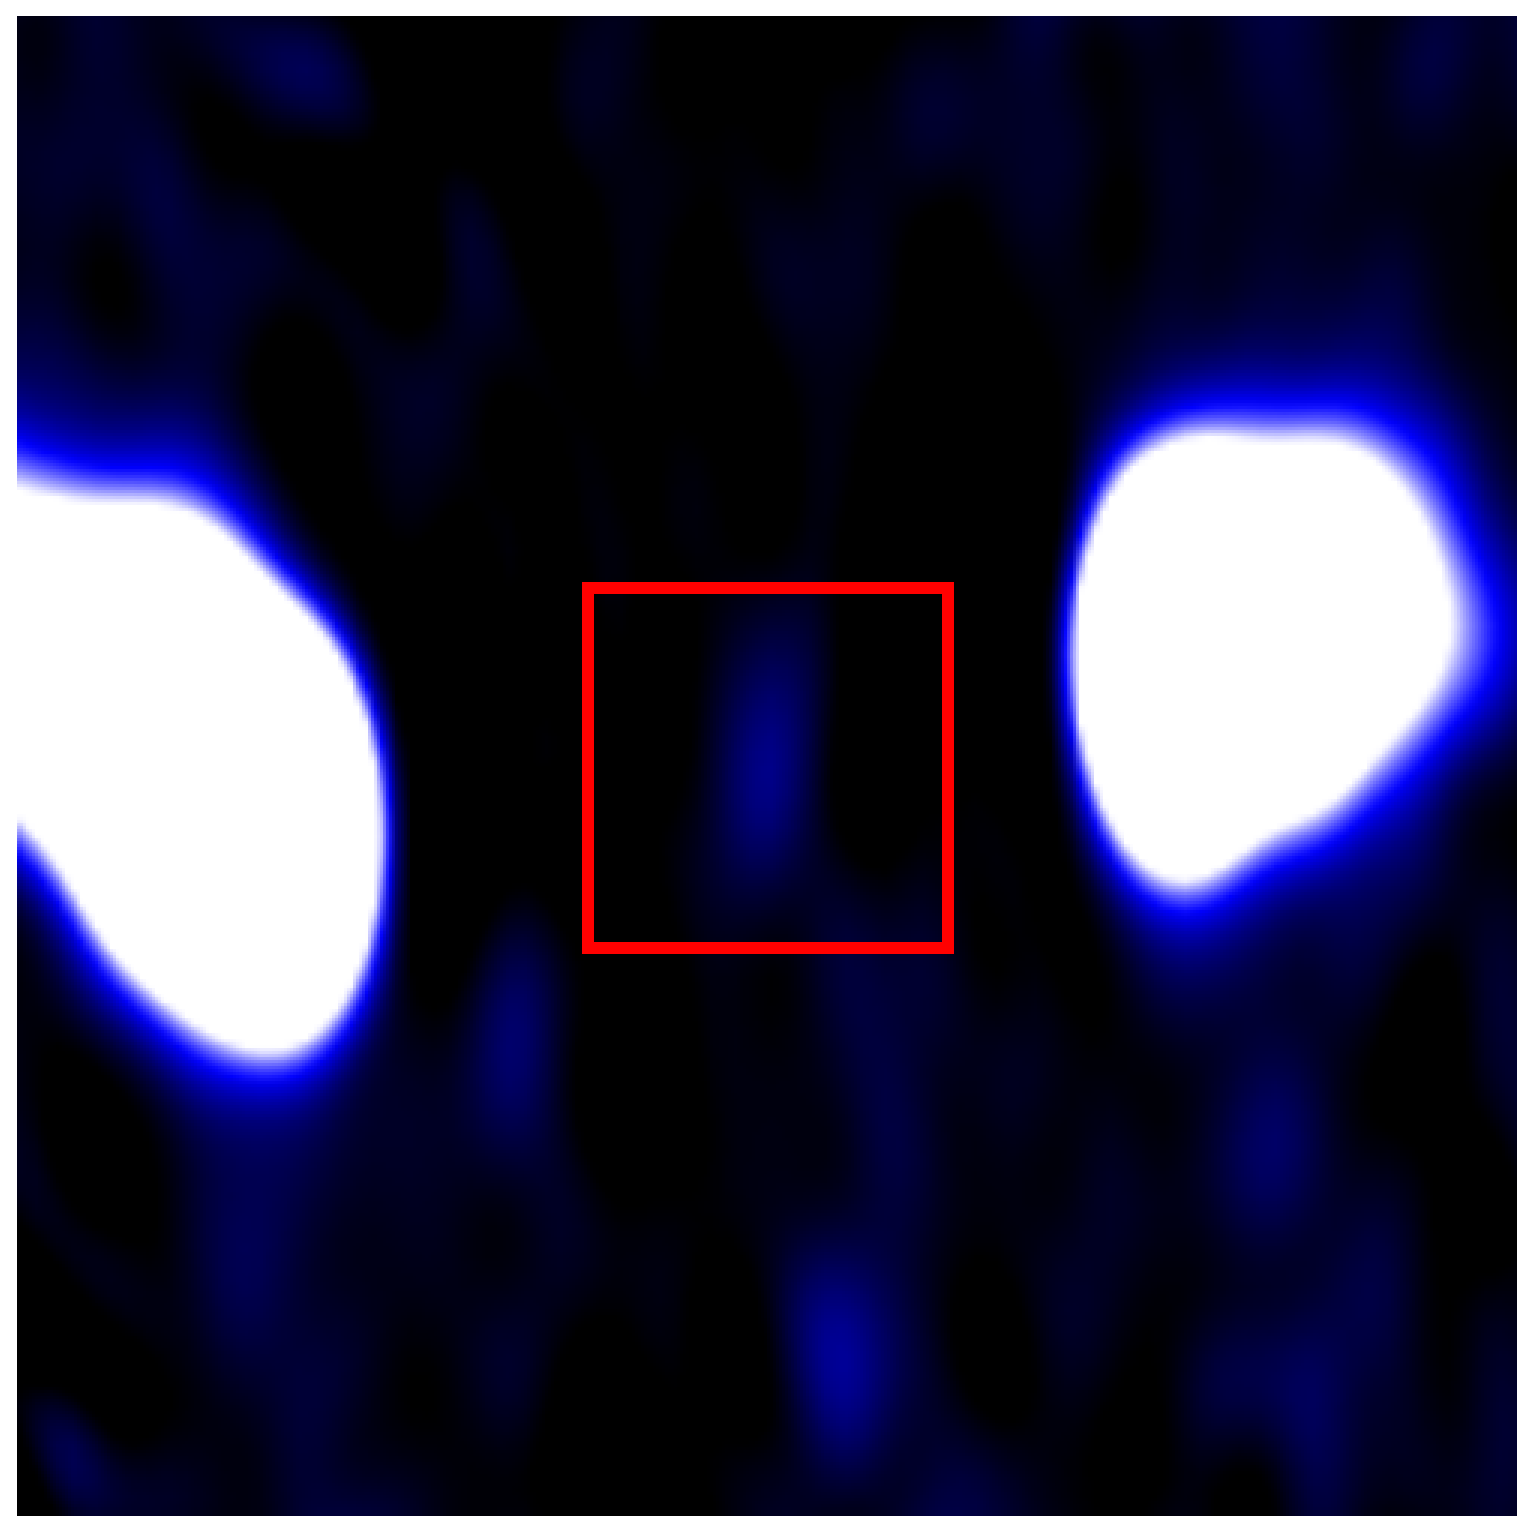
\includegraphics[width=0.5\linewidth]{images/ARG0003sky_radio.eps}
      \caption{A radio image centred on 03~26~39.12~$-$28~07~58.80.
        %ARG0003sky
        This is an example of a radio source where the window centred on the
        host galaxy, shown as a rectangle, does not contain enough radio
        information to correctly identify the galaxy as the host. [TODO: FITS, colour description, RA/Dec]}
      \label{fig:broken-window-size}
    \end{figure}

    A related issue is that we need to choose a window size for the image
    representations of each SWIRE object. If this image is too small, radio
    emission may extend past the edges of the window, and it may be impossible
    to identify the galaxy as a host galaxy. If the image is too large, then
    too much information will be included and it will be difficult or
    computationally expensive to classify. We chose a window size of $32
    \times 32$ pixels, shown as a red rectangle in Figures
    \ref{fig:windows} and \ref{fig:broken-window-size}.

    \begin{figure}
      \centering
      % http://www.texample.net/tikz/examples/simple-flow-chart/
      \tikzstyle{decision} = [diamond, draw, fill=white,
          text width=4.5em, text badly centered, inner sep=0pt]
      \tikzstyle{block} = [rectangle, draw, fill=white,
          text width=5em, text centered, rounded corners, minimum height=4em]
      \tikzstyle{line} = [draw, -latex']
      \begin{tikzpicture}[node distance=6mm, auto]
        \node [block] (init) {input radio source};
        \node [decision, right= of init] (iscompact) {compact?};
        \node [block, below= of iscompact] (compact) {find nearest infrared object};
        \node [block, right= of iscompact] (resolved) {find nearby infrared objects};
        \node [block, fill=black!10, right= of resolved] (classify) {classify objects};
        \node [block, below= of classify] (best) {find highest probability object};
        \coordinate (middle) at ($(compact)!0.5!(best)$);
        \node [block, below= of middle, fill=green!10] (done) {\textbf{host galaxy}};
        \path [line] (init) -- (iscompact);
        \path [line] (iscompact) -- (compact) node [midway] {yes};
        \path [line] (compact) -- (done);
        \path [line] (iscompact) -- (resolved) node [midway] {no};
        \path [line] (resolved) -- (classify);
        \path [line] (classify) -- (best);
        \path [line] (best) -- (done);
      \end{tikzpicture}
      \caption{A cross-identification method employing a binary classifier. As
        input we accept a radio source. If the source is compact, we select
        the nearest infrared object as the host galaxy. If the source is
        resolved, we classify all infrared objects nearby within radius $R$
        and select the highest probability object as the host galaxy. The grey
        box is the classifier, which can be any binary classifier that outputs
        a probability.}
      \label{fig:flowchart}
    \end{figure}

    We can improve upon this cross-identification method by filtering out
    compact radio sources, which are much easier to cross-identify --- the
    nearest SWIRE object may be identified as the host galaxy, or a more
    complex method such as likelihood ratios may be applied
    \citep[see][]{weston17}. A full cross-identification pipeline making use
    of this alongside a binary classifier is shown in Figure
    \ref{fig:flowchart}.

  \subsection{Vector representation of infrared
  sources}\label{vector-representation-of-infrared-sources}

  \cheng{I suggest not using the word ``vector''. Either ``feature vector'',
  or ``an array of real values''. Definitely not ``real valued vector''.}
    {[}TODO: Discuss comments on ``vector'' with Julie{]}

    Most binary classification methods require that the inputs to be
    classified are real-valued vectors. We thus need to choose a vector
    representation of our candidate host galaxies, also known as the
    ``features'' of the galaxies.

    {[}TODO: Add a plot of the SWIRE flux distributions along with the
    wedges{]}

    Infrared observations of the CDFS field are taken from SWIRE. We use the
    CDFS Fall '05 SWIRE catalogue \citep{surace05swire} to generate candidate
    hosts to classify. Radio observations of the CDFS field are taken from
    ATLAS. As almost all infrared sources in SWIRE look essentially the same
    (and differences in structure are likely irrelevant to whether the galaxy
    is a host galaxy), the candidate host location encodes almost all
    information we could gain from the infrared image. We therefore only use
    the radio image for object localisation.

    We represent each candidate host as 1034 real-valued features. For a given
    candidate host, these features are:
    \begin{itemize}
      \item the logarithm of the ratio of fluxes of the candidate host in the
        four IRAC wavelengths;
      \item the stellarity index of the host in both 3.6 $\mu$m and 4.5
        $\mu$m;
      \item the flux of the host in 3.6 $\mu$m;
      \item the radial distance between the candidate host and the nearest
        radio component in the ATLAS catalogue; and
      \item a 32 $\times$ 32 pixel image from ATLAS, centred on the candidate
        host.
    \end{itemize}

    [TODO: Cite Lacy 2004, 2010 or 2013 white paper, and rewrite this] The
    flux ratios are indicators of the star formation rate and amount of dust
    in the galaxy and might thus be predictors of whether the galaxy contains
    an AGN {[}Julie?{]} \ref{fig:magdiff}. The stellarity index represents how
    likely the object is to be a star rather than a galaxy.

  \subsection{Logistic regression}\label{logistic-regression}

    Logistic regression is the simplest classification model we can apply.
    It is linear in the feature space and outputs the probability that the
    input has a positive label. The model is

    \[
        f(\vec x) = \sigma(\vec w \cdot \vec x + b)
    \] where \(\vec w \in \mathbb{R}^D\) is a weights vector,
    \(b \in \mathbb{R}\) is a bias term, \(\vec x \in \mathbb{R}^D\) is the
    feature representation of a candidate host, and \(\sigma\) is the
    logistic sigmoid function \[
        \sigma(a) = (1 + \mathrm{exp}(-a))^{-1}.
    \]

    The logistic regression model is fully differentiable, and the weight vector $\vec w$ can therefore be learned by gradient methods.

  \subsection{Convolutional neural
  networks}\label{convolutional-neural-networks}

    Convolutional neural networks (CNNs) are a biologically-inspired
    prediction model for prediction with image inputs. A number of filters
    are convolved with an input image to produce output images called \emph{feature maps}, and these feature maps can then be convolved again with other filters on subsequent layers. This produces a network of convolutions. The whole network is
    differentiable with respect to the values of the filters, and so the
    filters can be learned by gradient methods. The final layer of the
    network is logistic regression, with the convolved outputs as input
    features. For more detail, see \citet[\S II.A][]{lecun98}.

    \begin{figure*}
      \centering
      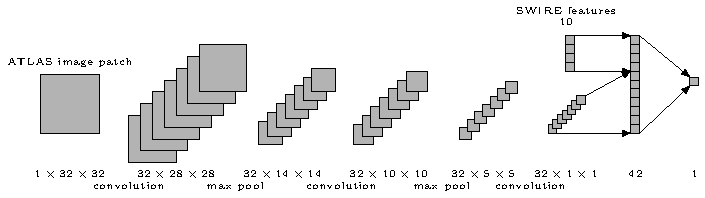
\includegraphics[width=\textwidth]{convnet.pdf}
      \caption{Convolutional neural network model.}
      \label{fig:cnn}
    \end{figure*}

    \begin{figure}
    \centering
    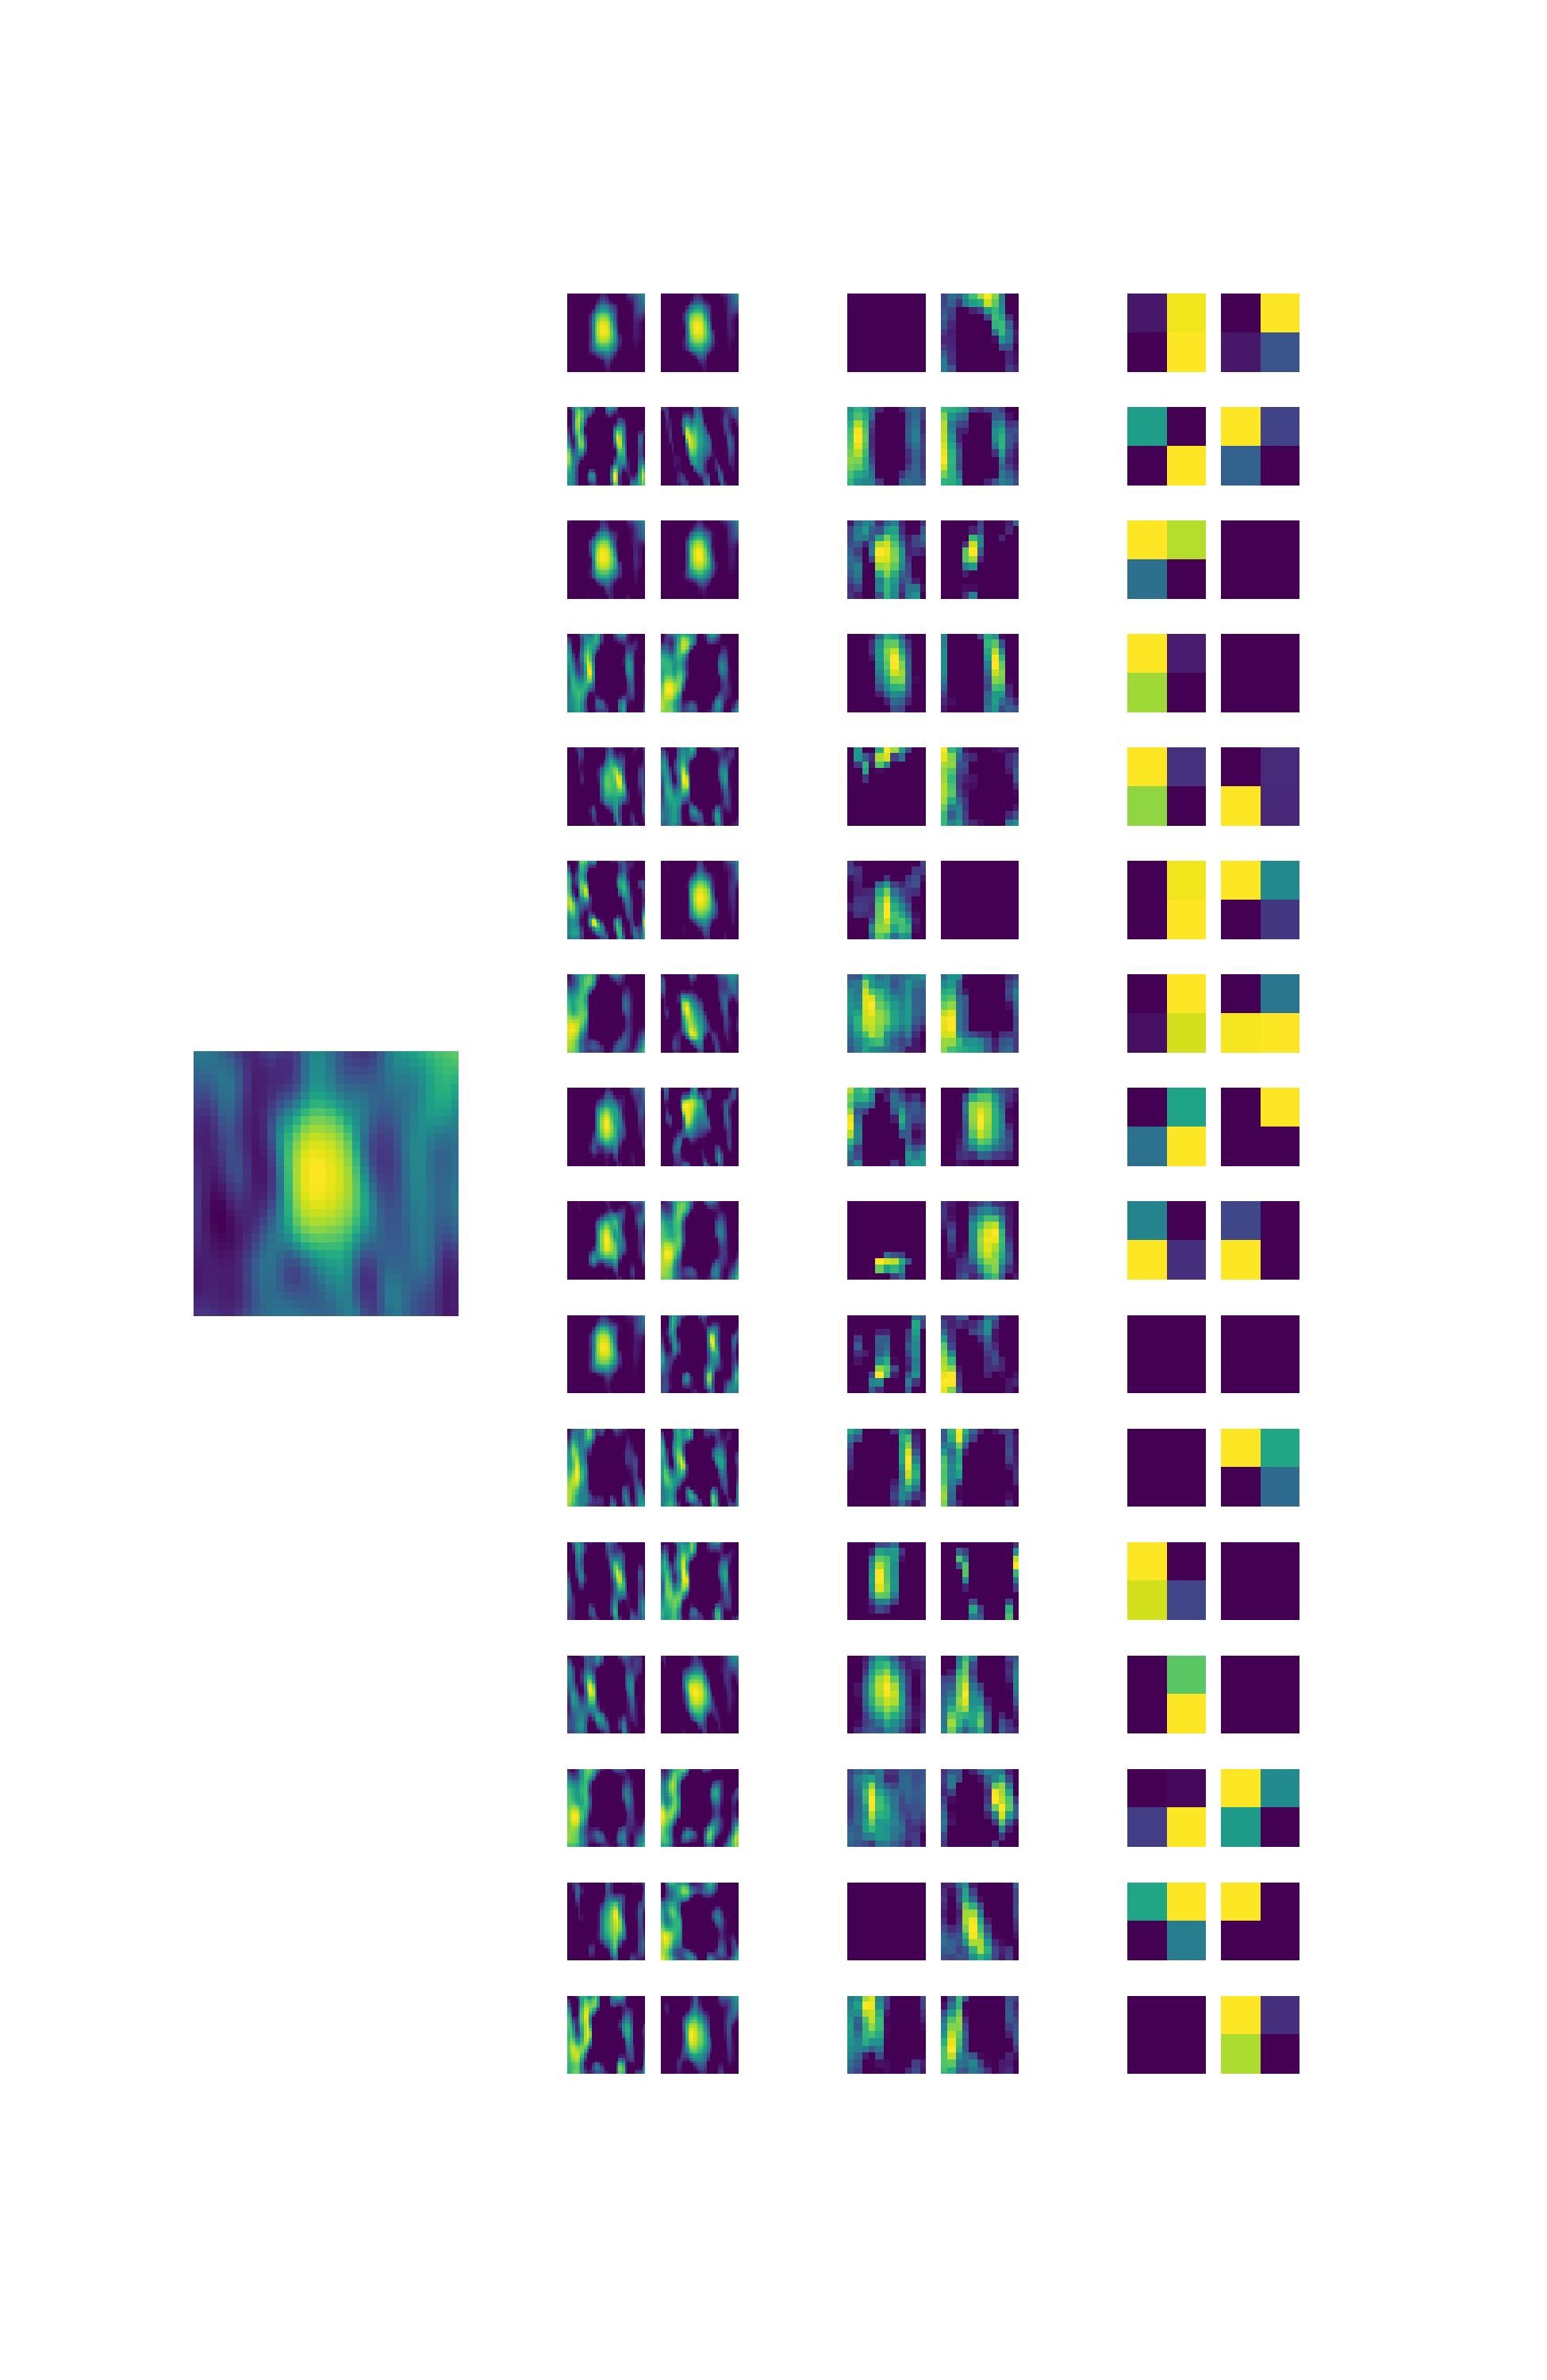
\includegraphics[width=0.6\columnwidth]{convolutions_42191.pdf}
    \caption{Feature maps from convolutional layers of a convolutional neural
      network trained on quadrants 1 -- 3 of CDFS with labels derived from
      \citeauthor{norris06} [TODO: Explain this diagram, add subfigures, maybe tidy it up a bit]}
    \label{fig:cnn-outputs}
    \end{figure}

    CNNs have recently produced good results on large image-based datasets [citation needed]. We employ only a simple CNN model in this paper
    --- CNNs can be arbitrarily complex --- as a proof of concept that CNNs
    may be used for prediction on radio images. The model we used is shown
    in Figure \ref{fig:cnn}. An example of this model reducing a radio image is shown in Figure \ref{fig:cnn-outputs}.

  \subsection{Random Forests}\label{random-forests}

    Random forests are an ensemble of decision trees~\citep{breiman01random-forest}.
    It considers multiple subsamples
    of the training set, where each bootstrap subsample is sampled with replacement
    from the training set. For each subsample a decision tree classifier is constructed,
    which builds an axis parallel split based on individual features in a greedy fashion.
    In a random forest the split decision is taken based on a random subset of features.
    For each test point, the random forest takes the weighted average of all the
    classifications produced by each decision tree.

  \subsection{Labels}\label{labels}

    Converting the Radio Galaxy Zoo and \citet{norris06} cross-identification
    catalogues to binary labels for infrared objects is a non-trivial task. A
    clear problem is that there is no way to capture radio morphology
    information in binary classification. As a result, we ignore this problem
    for this paper. Another problem is that there is no way to indicate
    \emph{which} radio object an infrared object is associated with, only that
    it is associated with \emph{some} radio object. We make the na\"ive
    assumption that any given radio image contains only one host galaxy as the
    first method in solving this problem.

    We then generate positive labels from a cross-identification catalogue.
    We decide that if an infrared object is listed in the catalogue, then it
    is assigned a positive label as a host galaxy. In principle we would
    then assign every other galaxy a negative label. This has some problems
    --- an example is that if the cross-identifier did not observe a radio
    object (e.g.~it was below the signal-to-noise ratio) then the host
    galaxy of that radio object would receive a negative label. {[}TODO:
    Count how many times this happens in Norris/RGZ.{]} This occurs with
    \citet{norris06} cross-identifications, as these are associated with
    the first data release of ATLAS. The first data release went to a depth
    of {[}TODO: depth of DR1{]}, compared to the depth of the third data
    release {[}TODO: depth of DR3{]} (Franzen et al. 2015) used by Radio
    Galaxy Zoo. Labels from Norris may therefore disagree with labels from
    Radio Galaxy Zoo even if they are both correct.

    There are many potential host galaxies {[}TODO: how many galaxies in
    SWIRE?{]}, so instead of using all galaxies in the CDFS field we only
    train and test our classifiers on infrared objects within a fixed radius
    of an ATLAS radio object. For this radius we choose \(1'\), the same
    radius as the images shown to volunteers in Radio Galaxy Zoo. In general
    this will result in cases where the host galaxy is outside the radius
    \citep[e.g. the giant radio galaxy shown in][]{banfield15}, but this is
    unavoidable. We may also choose a radius which is too \emph{large},
    worsening our assumption that there is only one host galaxy in this
    radius, but again, this is unavoidable.

    {[}How badly does this assumption hurt us? How does a perfect binary
    classifier behave under these assumptions?{]}

    (TODO: Describe how we assigned labels given that RGZ only labels the
    first component.)

  \subsection{Experimental Setup}\label{experimental-setup}

    \begin{figure}
      \centering
      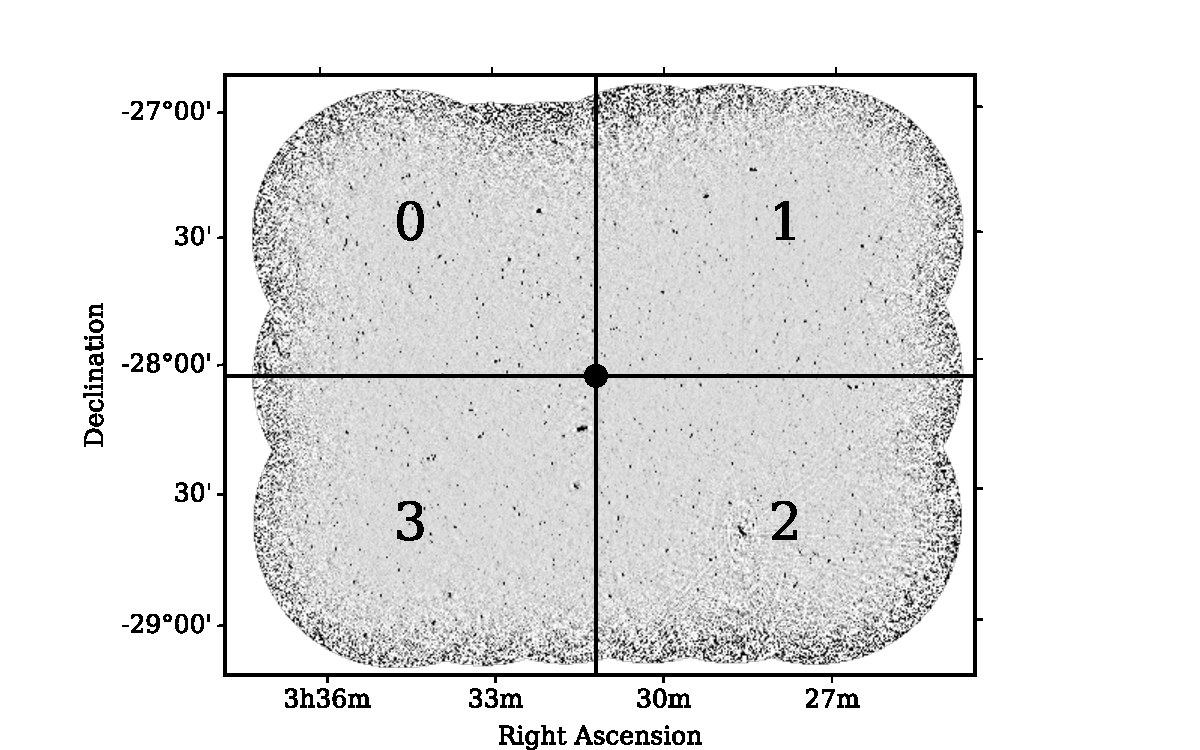
\includegraphics[width=\columnwidth]{images/quadrants.pdf}
      \caption{CDFS field training and testing quadrants. The central dot is
        located at 52h48m00s -28$^\circ$06m00s. There are similar numbers of
        radio sources in each quadrant.\label{fig:quadrants}}
    \end{figure}

    We trained cross-identifiers on radio objects from the ATLAS
    observations of the Chandra Deep Field - South (CDFS) using Radio Galaxy
    Zoo cross-identifications, and compared the trained cross-identifiers to
    those trained on a set of expert cross-identifications of the same
    field. We then applied the cross-identifiers trained on CDFS to the ESO
    Large Area ISO Survey - South 1 (ELAIS-S1) field {[}TODO{]}.

    We divided the CDFS field into four quadrants for training and testing.
    The quadrants were centred on 52h48m00s -28$^\circ$06$'$00$''$
    (Figure \ref{fig:quadrants}). For each trial, one quadrant
    was used to draw test examples, and the other three quadrants were used
    for training examples.

    We further divided the radio components into compact and resolved. Compact
    components are trivially cross-identified by fitting a 2D Gaussian \citep[as
    in][]{norris06} and we would expect any machine learning approach for host
    cross-identification to attain high accuracy on this set. Whether a
    component was resolved was decided based on its flux; a radio component
    was considered resolved if
    \[
        \ln \left(
          \frac{S_{\text{int}}}
               {S_{\text{peak}}}
        \right) > 2\sqrt{\left(
          \frac{\sigma_{S_{\text{int}}}}
               {S_{\text{int}}}
        \right)^2 + \left(
          \frac{\sigma_{S_{\text{peak}}}}
               {S_{\text{peak}}}
        \right)^2},
    \] and compact otherwise, where \(S_{\text{int}}\) is the integrated
    flux and \(S_{\text{peak}}\) is the peak flux \citep{franzen15}.

    We considered only radio objects with a cross-identification in both the
    \citet{norris06} catalogue and the RGZ catalogue. Candidate hosts
    were then selected from the SWIRE catalogue. For a given subset of radio
    objects, all SWIRE objects within $1'$ of all radio objects in the
    subset were added to the associated SWIRE subset.

    Each classifier was trained on the training examples and used to predict
    labels for the test examples. The predicted labels were compared to the
    labels derived from the \citet{norris06} cross-identifications and the
    balanced accuracy was computed. We used balanced accuracy as our accuracy
    measure due to the highly imbalanced classes --- in our total set of SWIRE
    objects within $1'$ of an ATLAS object, only 4\% have positive labels.
    Only examples within $1'$ of ATLAS objects in the first ATLAS data release
    \citep{norris06} were used to compute accuracy, as these were the only
    ATLAS objects with \citet{norris06} labels. We report the balanced
    accuracy on the classification task for logistic regression, convolutional
    neural networks, and random forests. We also report the predictions for
    each SWIRE object. The reported predictions for a given object are made by
    classifiers tested on the quadrant containing that object.

    We then used the outputs of our classifiers to predict the host galaxy
    for each radio component cross-identified by both \citet{norris06}
    and Radio Galaxy Zoo. For each SWIRE object within $1'$ of the radio
    component, the probability of the object having a positive label was
    estimated using the trained binary classifiers. The SWIRE object with
    the highest probability was chosen as the host galaxy. The accuracy was
    then estimated by counting how many predicted host galaxies matched the
    \citet{norris06} cross-identifications. We report the accuracies and the
    cross-identifications. As with SWIRE predictions, reported
    cross-identifications for a given object are made by classifiers tested
    on the quadrant containing that object.

    The balanced accuracy provides a good proxy to the accuracy of the host
    cross-identification task. To check this, we selected random, small
    subsets of the SWIRE training objects, and for each random subset trained
    a logistic regression classifier. The balanced accuracy of this classifier
    was computed and compared with the accuracy of this classifier on the host
    cross-identification task. These accuracies are plotted against each other
    in Figure \ref{fig:gct-to-xid}. We found a positive correlation.
    Additionally, we compared the balanced accuracy of the classifier to the
    mean distance of the predicted host galaxy from the true host galaxy, also
    finding a positive correlation. [TODO: Quantify the correlation.]

\section{Results}\label{results}

  {[}TODO: Include images of ``good'' and ``bad'' X-IDs/GCTs.{]}
  \begin{figure}
  \centering
  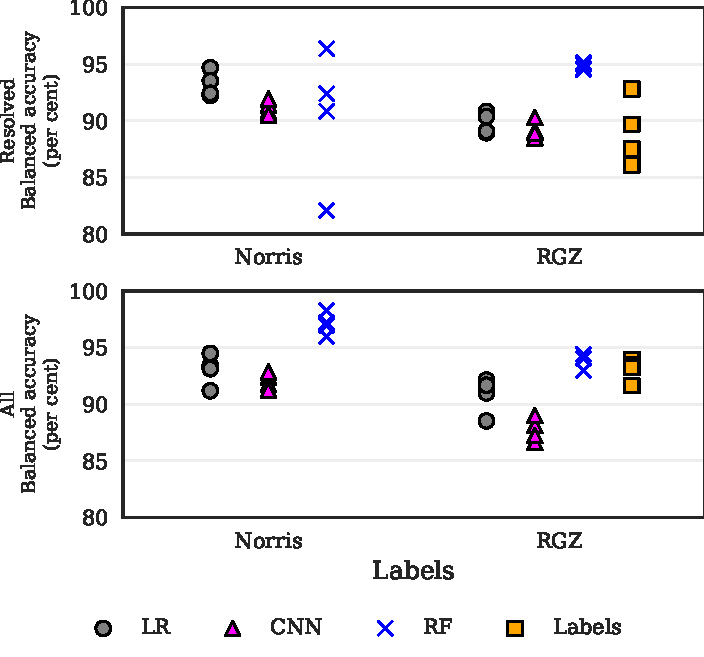
\includegraphics[width=\columnwidth]{images/cdfs_ba_grid.pdf}
  \caption{Balanced accuracies for each quadrant in the galaxy
    classification task. The maximum attainable balanced accuracy
    is 100\%, when every galaxy label matches the labels derived
    from \citet{norris06} cross-identifications.\label{fig:ba}}
  \end{figure}

  \begin{figure}
  \centering
  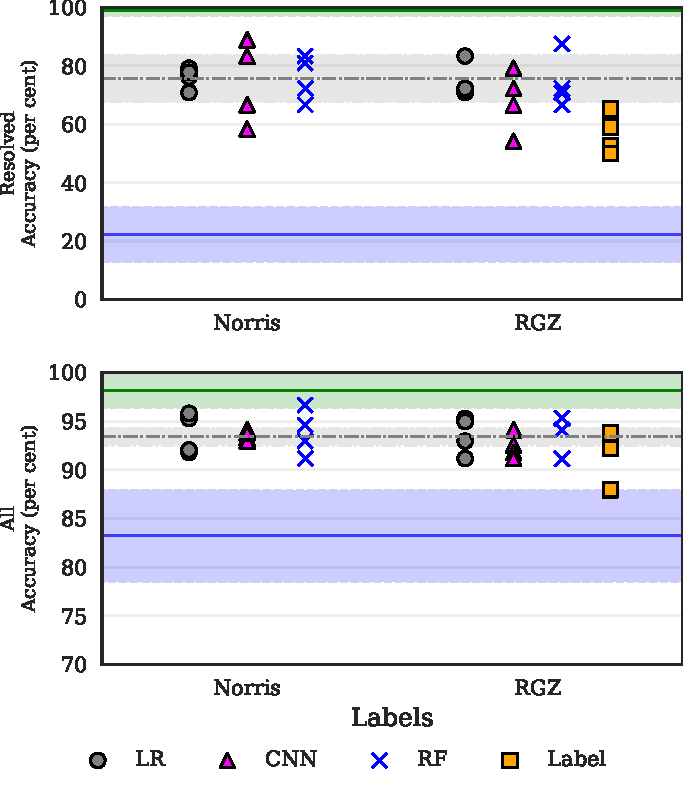
\includegraphics[width=\columnwidth]{images/cdfs_cross_identification_grid.pdf}
  \caption{Accuracies for each quadrant in the cross-identification
    task. The horizontal line indicates the accuracy of a "perfect" classifier
    on the cross-identification task, with the dashed lines indicating the
    standard deviation across CDFS quadrants. A "perfect" classifier simply
    reads the correct labels, in this case the labels derived from
    \citet{norris06}. This represents the maximum attainable cross-identification
    accuracy under our assumptions.
    \label{fig:cross-id-accuracy}}
  \end{figure}

  \cheng{Generate results and plots for accuracy, for the supplement}

  \begin{table*}
    \begin{tabular}{cccccccccccccccccccccccccccccc}
      SWIRE & RA & Dec & CNN(Norris / All) & CNN(Norris / Compact) & \dots & RF(RGZ N / Resolved) \\\hline
      SWIRE3\textunderscore J032559.15-284724.2 & 51.4965 & -28.7901 & 0.0001 & 0.3585 & \dots & 0.2815 \\
      SWIRE3\textunderscore J032559.91-284728.9 & 51.4996 & -28.7914 & 0.0004 & 0.3909 & \dots & 0.0000 \\
      SWIRE3\textunderscore J032600.02-284736.9 & 51.5001 & -28.7936 & 0.0002 & 0.3395 & \dots & 0.0000 \\
      SWIRE3\textunderscore J032600.13-284637.5 & 51.5005 & -28.7771 & 0.0004 & 0.4546 & \dots & 0.0696 \\
      SWIRE3\textunderscore J032600.13-284715.7 & 51.5006 & -28.7877 & 0.0014 & 0.3857 & \dots & 0.0000 \\
      SWIRE3\textunderscore J032600.98-284705.4 & 51.5041 & -28.7848 & 0.0205 & 0.3742 & \dots & 0.0000 \\
      SWIRE3\textunderscore J032601.03-284711.6 & 51.5043 & -28.7866 & 0.0699 & 0.3752 & \dots & 0.0000 \\
      SWIRE3\textunderscore J032601.56-284131.0 & 51.5065 & -28.692 & 0.0001 & 0.3917 & \dots & 0.0819 \\
      SWIRE3\textunderscore J032601.60-284207.5 & 51.5067 & -28.7021 & 0.0000 & 0.3182 & \dots & 0.0000 \\
    \end{tabular}
    \caption{Predicted probabilities that each object in SWIRE is a host
      galaxy. Probabilities are reported for each predictor. C(A / B) indicates
      the predictor using classifier model C, trained on label set A on data set
      B. If a SWIRE object does not appear in the table, then it was further
      than $1'$ from an ATLAS object and hence has a predicted probability of
      zero by our assumptions. Full table electronic.}
    \label{tab:probs}
  \end{table*}

  \begin{table*}
    \small
    \begin{tabular}{ccccccccccc}
      SWIRE & RA & Dec & Norris & RGZ & RGZ radio consensus \\\hline
      ATLAS3\textunderscore{}J032602.82-284708.1C & 51.511734 & -28.785575 & SWIRE3\textunderscore{}J032603.15-284708.5 & & 0.4516\\
      ATLAS3\textunderscore{}J032615.49-284629.4C & 51.564555 & -28.774847 & SWIRE3\textunderscore{}J032615.41-284630.7 & SWIRE3\textunderscore{}J032615.41-284630.7 & 0.2941\\
      ATLAS3\textunderscore{}J032615.55-280559.8C & 51.564799 & -28.099955 & SWIRE3\textunderscore{}J032615.52-280559.8 & SWIRE3\textunderscore{}J032615.52-280559.8 & 0.5625\\
      ATLAS3\textunderscore{}J032617.35-280710.2C & 51.572279 & -28.119491 & SWIRE3\textunderscore{}J032617.89-280707.2 & SWIRE3\textunderscore{}J032617.89-280707.2 & 0.4146\\
      ATLAS3\textunderscore{}J032625.13-280909.8C & 51.604711 & -28.152731 & SWIRE3\textunderscore{}J032625.19-280910.1 & SWIRE3\textunderscore{}J032625.19-280910.1 & 0.3158\\
      ATLAS3\textunderscore{}J032629.10-280650.1C & 51.621251 & -28.113924 & SWIRE3\textunderscore{}J032629.13-280650.7 & SWIRE3\textunderscore{}J032626.74-280636.7 & 0.3333\\
      ATLAS3\textunderscore{}J032629.61-284052.7C & 51.623385 & -28.681315 & SWIRE3\textunderscore{}J032629.54-284055.8 & SWIRE3\textunderscore{}J032629.54-284055.8 & 0.2676\\
      ATLAS3\textunderscore{}J032629.92-284753.5C & 51.624653 & -28.798195 & SWIRE3\textunderscore{}J032629.81-284754.4 & SWIRE3\textunderscore{}J032629.81-284754.4 & 1.0000\\
      ATLAS3\textunderscore{}J032630.66-283657.3C & 51.62777 & -28.615917 & SWIRE3\textunderscore{}J032630.64-283658.0 & SWIRE3\textunderscore{}J032628.56-283744.8 & 0.3611
    \end{tabular}
    \begin{tabular}{ccccc}
      RGZ IR consensus & CNN(Norris / All) & CNN(Norris / Compact) & \dots & RF(RGZ N / Resolved) \\\hline
      0.3214 & SWIRE3\textunderscore{}J032602.36-284711.5 & SWIRE3\textunderscore{}J032602.36-284711.5 & \dots & SWIRE3\textunderscore{}J032603.60-284627.4 \\
      0.8000 & SWIRE3\textunderscore{}J032615.41-284630.7 & SWIRE3\textunderscore{}J032615.41-284630.7 & \dots & SWIRE3\textunderscore{}J032615.41-284630.7 \\
      0.8333 & SWIRE3\textunderscore{}J032615.52-280559.8 & SWIRE3\textunderscore{}J032615.52-280559.8 & \dots & SWIRE3\textunderscore{}J032615.52-280559.8 \\
      1.0000 & SWIRE3\textunderscore{}J032617.89-280707.2 & SWIRE3\textunderscore{}J032617.89-280707.2 & \dots & SWIRE3\textunderscore{}J032616.86-280715.8 \\
      0.6667 & SWIRE3\textunderscore{}J032625.19-280910.1 & SWIRE3\textunderscore{}J032625.19-280910.1 & \dots & SWIRE3\textunderscore{}J032625.19-280910.1 \\
      1.0000 & SWIRE3\textunderscore{}J032629.13-280650.7 & SWIRE3\textunderscore{}J032629.13-280650.7 & \dots & SWIRE3\textunderscore{}J032629.13-280650.7 \\
      1.0000 & SWIRE3\textunderscore{}J032629.13-280650.7 & SWIRE3\textunderscore{}J032629.13-280650.7 & \dots & SWIRE3\textunderscore{}J032629.13-280650.7 \\
      0.8571 & SWIRE3\textunderscore{}J032629.81-284754.4 & SWIRE3\textunderscore{}J032629.81-284754.4 & \dots & SWIRE3\textunderscore{}J032629.81-284754.4 \\
      0.7308 & SWIRE3\textunderscore{}J032630.64-283658.0 & SWIRE3\textunderscore{}J032628.56-283744.8 & \dots & SWIRE3\textunderscore{}J032628.56-283744.8
    \end{tabular}
    \caption{Predicted host galaxy cross-identifications for each object in
      ATLAS-CDFS. Cross-identifications are reported for each predictor, with
      the predictor listed as in Table \ref{tab:probs}. The cross-identification
      given by \citet{norris06} is included in the "Norris" column. The
      cross-identification given by the Radio Galaxy Zoo consensus is included in
      the "RGZ" column, along with the corresponding consensus levels for the radio
      morphology and host cross-identification tasks. Low radio consensus
      indicates that the component has multiple nearby components (and thus is
      more impacted by our assumption that the source is isolated), and low
      infrared consensus indicates that the host galaxy is unclear in the SWIRE
      image (possibly due to multiple nearby candidate host galaxies). Full table
      electronic. \cheng{What is consensus?}}
    \label{tab:cids}
  \end{table*}

  \begin{figure}
  \centering
  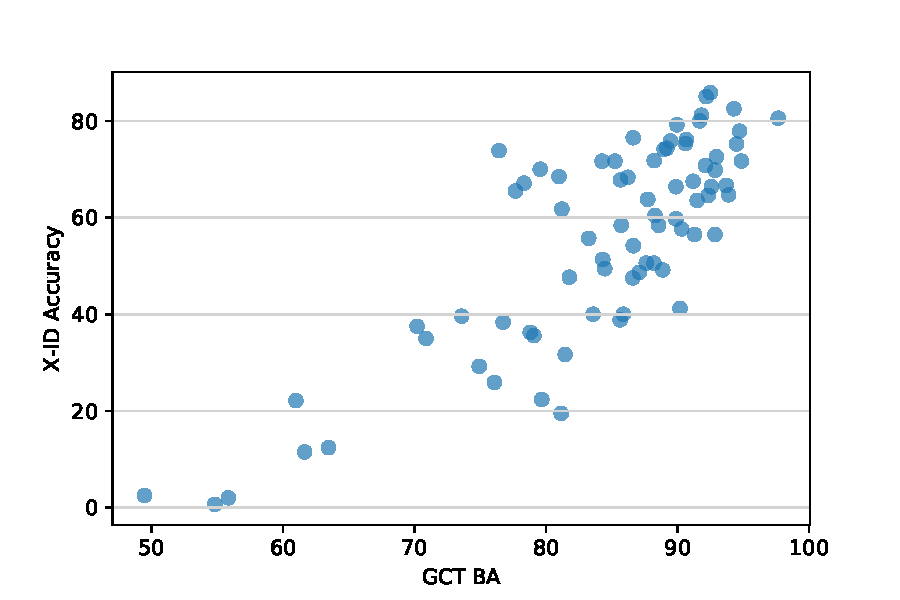
\includegraphics[width=\columnwidth]{gct-to-xid.pdf}
  \caption{Classification balanced accuracy against accuracy on the
  cross-identification task. Cross-identification accuracy is computed
  from a binary comparison between the predicted host and the Norris et
  al. (2006) cross-identification; neither distance to the true host nor
  broken assumptions of one host per image are accommodated. {[}TODO:
  explain this caption better so that it is understandable to non-ML
  people; regenerate this with the new pipeline{]}\label{fig:gct-to-xid}}
  \end{figure}

  % \begin{figure}
  % \centering
  % 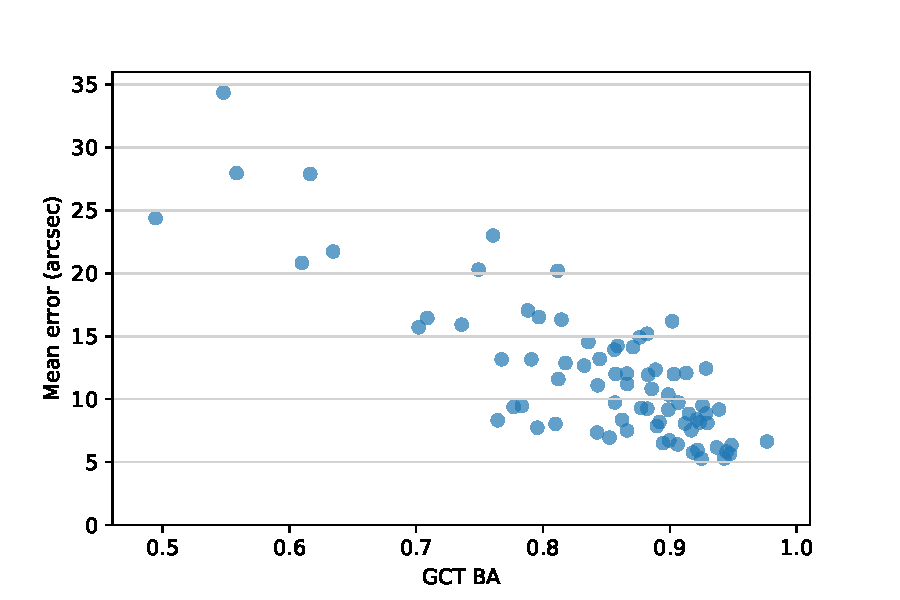
\includegraphics[width=\columnwidth]{gct-to-arcsec-error.pdf}
  % \caption{Classification balanced accuracy against average radial
  % distance between the predicted and the \citet{norris06} cross-identified
  % host on the cross-identification task.\label{fig:gct-to-arcsec-error}}
  % \end{figure}

  \begin{figure}
  \centering
  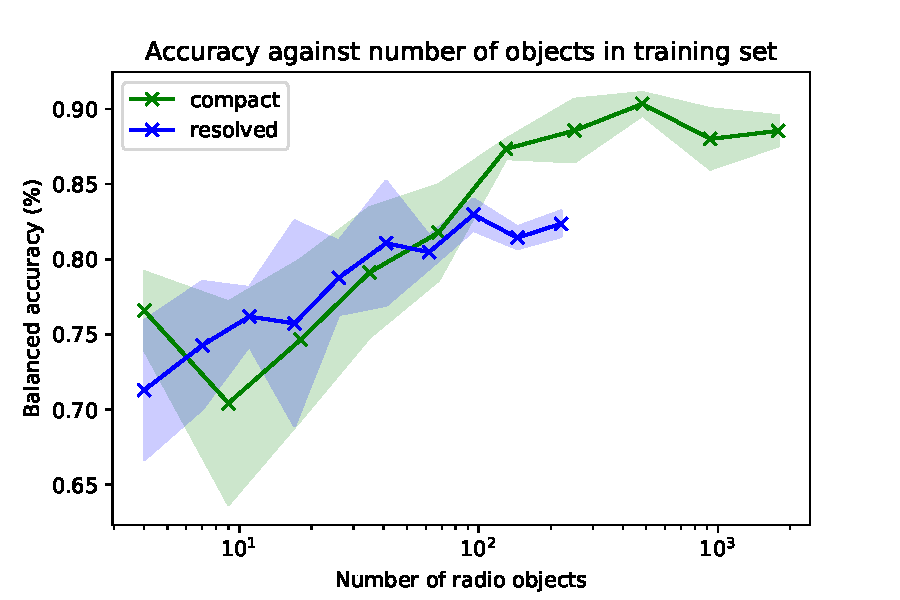
\includegraphics[width=\columnwidth]{passive.pdf}
  \caption{Passive learning plot for the GCT. Trained and tested on RGZ.
    This is so that we had maximal training data --- RGZ has many more
    objects than Norris. [TODO: Regenerate with Norris testing data]
    \label{fig:passive}}
  \end{figure}

  \begin{figure}
  \centering
  
\includegraphics[width=\columnwidth]{distributions.pdf}
  \caption{Distribution of non-image features.\label{fig:distributions}}
  \end{figure}

  \begin{figure*}
    \subfloat{\includegraphics[width=0.45\linewidth]{images/examples/\detokenize{CNN_Norris_ATLAS3_J032629.61-284052.7C}.pdf}}\hspace{1cm}
    \subfloat{\includegraphics[width=0.45\linewidth]{images/examples/\detokenize{CNN_Norris_ATLAS3_J032824.66-274149.7C}.pdf}}\\
    \subfloat{\includegraphics[width=0.45\linewidth]{images/examples/\detokenize{CNN_Norris_ATLAS3_J032908.32-284827.0C}.pdf}}\hspace{1cm}
    \subfloat{\includegraphics[width=0.45\linewidth]{images/examples/\detokenize{CNN_Norris_ATLAS3_J032916.31-272341.2C}.pdf}}\\
  \end{figure*}
  \begin{figure*}
    \subfloat{\includegraphics[width=0.45\linewidth]{images/examples/\detokenize{CNN_Norris_ATLAS3_J033022.32-272121.1C}.pdf}}\hspace{1cm}
    \subfloat{\includegraphics[width=0.45\linewidth]{images/examples/\detokenize{CNN_Norris_ATLAS3_J033242.02-273818.8C}.pdf}}\\
    \subfloat{\includegraphics[width=0.45\linewidth]{images/examples/\detokenize{CNN_Norris_ATLAS3_J033433.94-271812.9C}.pdf}}\hspace{1cm}
    \subfloat{\includegraphics[width=0.45\linewidth]{images/examples/\detokenize{CNN_Norris_ATLAS3_J033436.18-272632.0C}.pdf}}\\
  \end{figure*}

  \begin{figure}
  \centering
  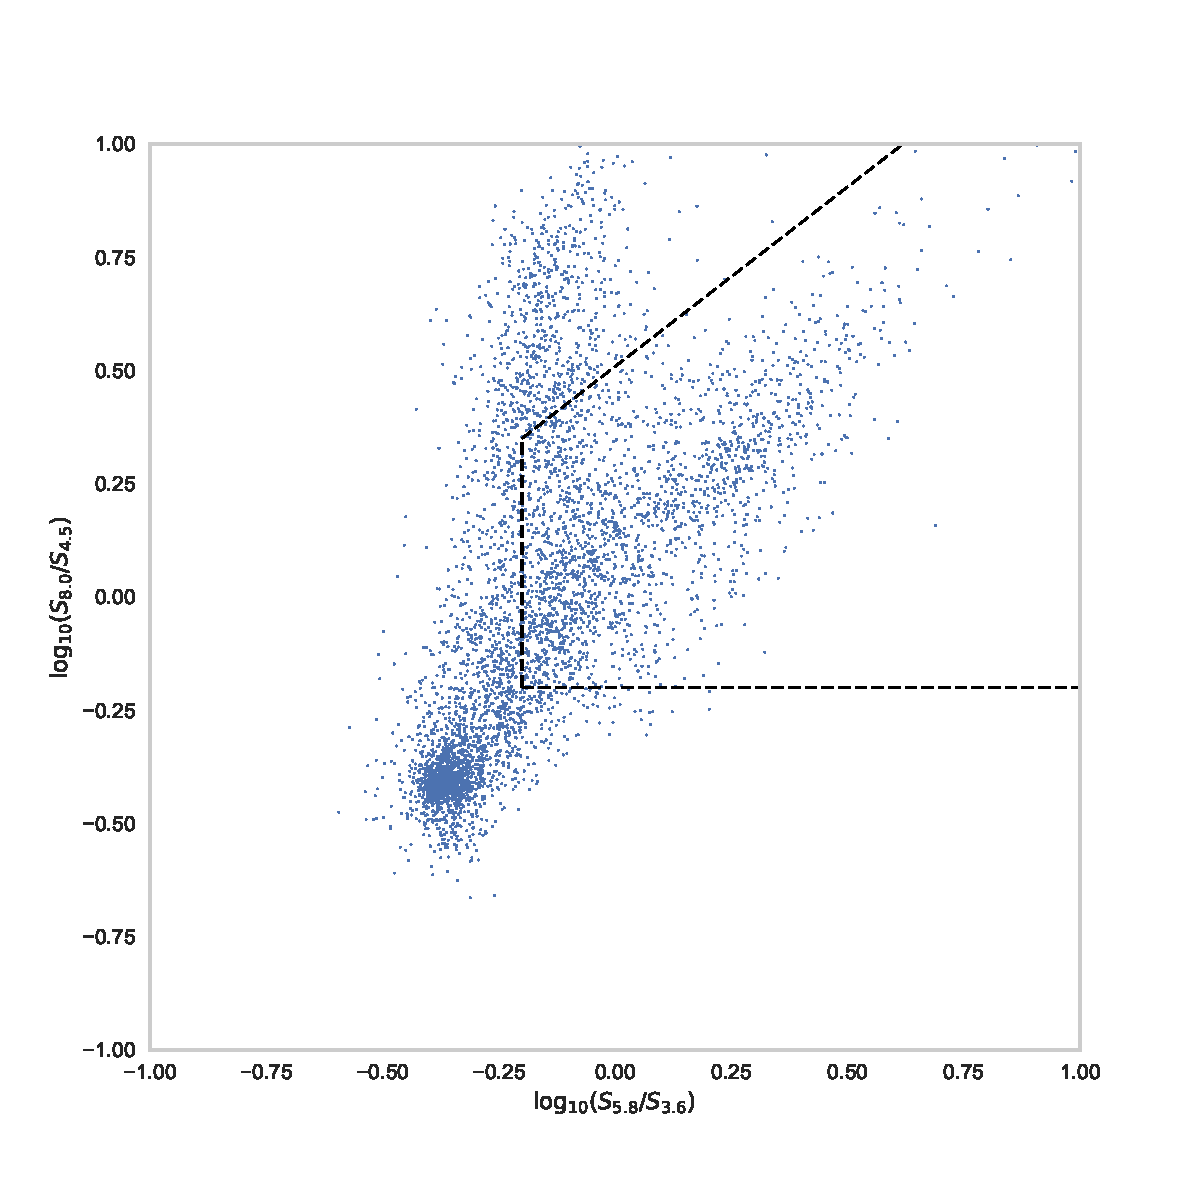
\includegraphics[width=\columnwidth]{colour-colour-all.pdf}
  \caption{Colour-colour diagram for sample of SWIRE objects within \(R\)
  of an ATLAS object.\label{fig:colour-colour-all}}
  \end{figure}

  \begin{figure}
  \centering
  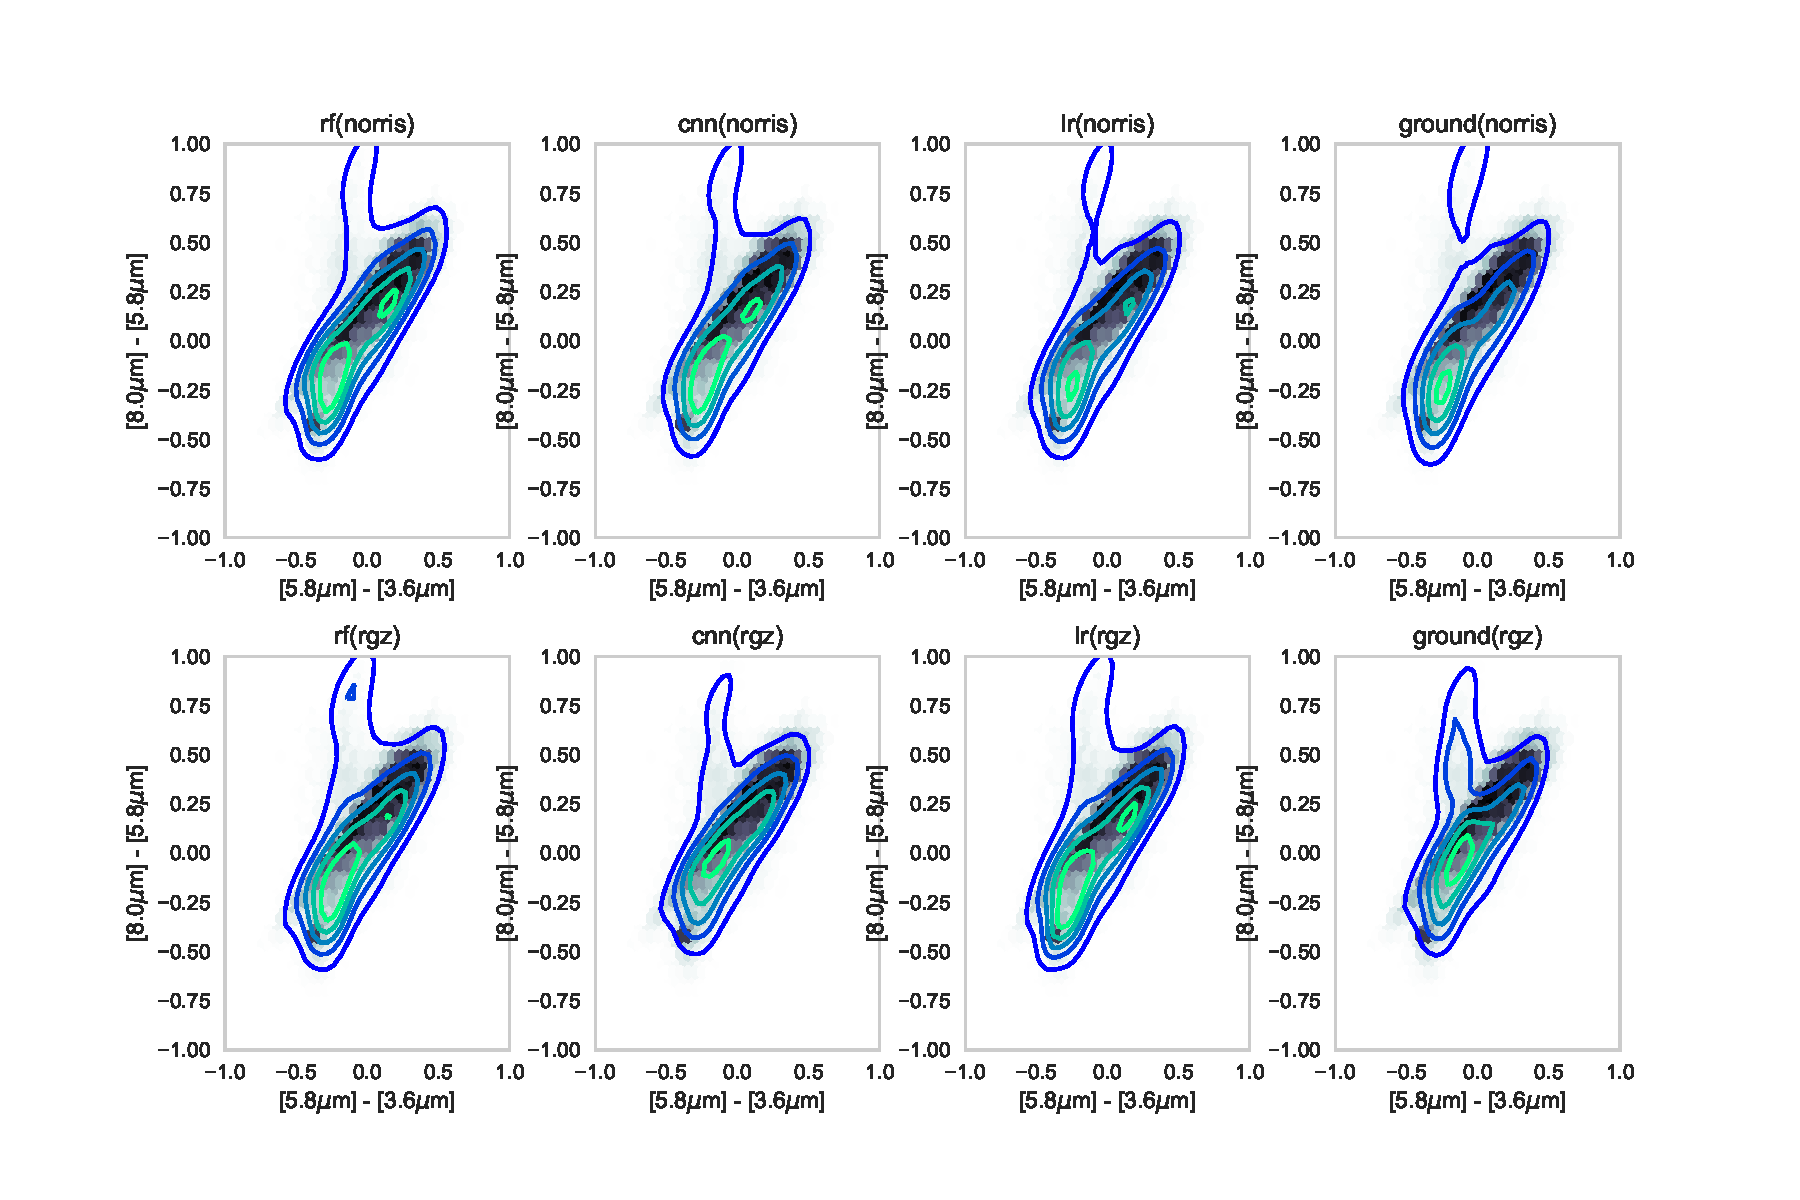
\includegraphics[width=\columnwidth]{colour_colour_predictions.pdf}
  \caption{Colour-colour diagrams for each
  classifier.\label{fig:colour-colour}}
  \end{figure}

  {[}TODO: Axis labels should say e.g. \(\log_{10}(S_{5.8}/S_{3.6})\);
  include the SWIRE wedges from Lacy et al. 2004.{]}

\section{Application to ATLAS-ELAIS}

\section{Summary}
%
%%%%%%%%%%%%%%%%%%%% REFERENCES %%%%%%%%%%%%%%%%%%
\bibliographystyle{mnras}
\bibliography{rgz-cdfs-ms}

%%%%%%%%%%%%%%%%%%%%%%%%%%%%%%%%%%%%%%%%%%%%%%%%%%


% Don't change these lines
\bsp	% typesetting comment
\label{lastpage}
\end{document}
